\documentclass[a4paper,12pt]{article}
\usepackage{silence}
\WarningFilter{fancyhdr}{\headheight is too small}

% Packages
\usepackage[utf8]{inputenc}
\usepackage{graphicx}
\usepackage{hyperref}
\usepackage{geometry}
\geometry{margin=1in}
\usepackage{titlesec}
\usepackage{fancyhdr}
\usepackage{listings}
\usepackage{longtable}
\usepackage{hyperref}
\hypersetup{
  pdfauthor={Parakram},
  pdftitle={Lab 1 Report: HTML/CSS-based Product Catalog},
  pdfsubject={Ecommerce},
  pdfcreator={Parakram},      
  pdfproducer={pdfLaTeX}  
}

\usepackage{booktabs}
\usepackage{xcolor}
\usepackage{colortbl}
\usepackage{setspace}
\usepackage{lmodern}
% For listing colors
%\usepackage{datetime} % For formatting date
%\usepackage{listings-css} % Adds CSS language support to listings

% Customize listings appearance

\lstset{
  basicstyle=\ttfamily\small,
  keywordstyle=\color{blue},
  stringstyle=\color{red},
  commentstyle=\color{green!50!black},
  breaklines=true,
  frame=single,
  numbers=left,
  numberstyle=\tiny,
  stepnumber=1,
  numbersep=5pt,
  showstringspaces=false,
  tabsize=2,
}
\lstdefinelanguage{CSS}{
  morekeywords={color, background, font-size, margin, padding, border, float, width, height, text-align,overflow,position, object-fit, transition,box-shadow },
  sensitive=true,
  morecomment=[l]{//},
  morestring=[b]",
}
% Header and footer setup for all pages except cover
\fancypagestyle{main}{
  \fancyhf{}
  \rhead{CSC381 - E-Commerce}
  \lhead{Lab 1: Product Catalog}
  \cfoot{\thepage}
  \renewcommand{\headrulewidth}{0.4pt}
  \renewcommand{\footrulewidth}{0.4pt}
}

\title{Lab Report 1: HTML/CSS-based Product Catalog}
\author{Submitted by: Parakram Kharel \\ Roll No: 24 \\ 
\textit{Kathford International College of Engineering and Management} \\ 
Affiliated to Tribhuvan University}
% \date{\today}
\makeatletter
\begin{document}
% \date{August 17, 2025}


% --------- Cover Page ---------
\begin{titlepage}
  \begin{center}
    \vspace*{2cm}
    
\includegraphics[width=0.35\textwidth]{Kath.png} \\[2cm]

    {\Huge \bfseries Lab Report 1} \\[0.5cm]
    {\Large HTML/CSS-based Product Catalog} \\[2cm]

    {\Large \textbf{Course:} CSC381 - E-Commerce} \\[1cm]
    {\Large \textbf{Submitted by:}} \\[0.3cm]
    {\large Parakram Kharel \\ Roll No: 24} \\[2cm]

    \textit{Kathford International College of Engineering and Management} \\
    Affiliated to Tribhuvan University \\[3cm]
    
    \date{August 17, 2025}
    {\normalsize \@date}
    % \today
  \end{center}
\end{titlepage}

\pagestyle{main}
\setlength{\parskip}{1em}

\section*{1. Objective}
To create and build a simple product catalog web page using HTML and CSS to display e-commerce product listings, focusing on layout, design, and structure.


\section*{2. Tools and Technologies Used}
\begin{longtable}{ll}
\toprule
\textbf{Technology} & \textbf{Purpose} \\
\midrule
HTML5 & Structure and layout of the web page \\
CSS3 & Styling and visual design \\
VS Code & Code editor and development environment \\
Web Browser & Rendering and testing output \\
\bottomrule
\end{longtable}

\section*{3. Theory / Background}
A product catalog page on an e-commerce site showcases the available products, featuring their images, names, prices, and short descriptions. HTML provides the structure and elements of the page, while CSS improves its visual style, layout, and responsiveness.

\section*{4. Page Layout Design}
\subsection*{4.1 Catalog Page Structure}
\begin{itemize}
  \item Header (website title or logo)
  \item Product grid with multiple product entries
  \item Footer with contact or legal information
\end{itemize}

\subsection*{4.2 Product Card Format}
Each product listing contains:
\begin{itemize}
  \item Product Image
  \item Product Title
  \item Brief Description of Product
  \item Price in NPR
\end{itemize}

\section*{5. Code Snippets}
\subsection*{5.1 HTML Code: Product Cart }
\begin{lstlisting}[language=HTML]
<div class="product-card" data-category="electronics">
    <div class="product-image">
        <img src="images/headphone.jpg" alt="Wireless Headphones">
        <div class="product-badge">NEW</div>
    </div>
    <div class="product-info">
        <h3>Premium Headphones</h3>
        <p class="product-desc">High-quality wireless headphones with noise cancellation</p>
        <div class="price-tag">NPR 8,999</div>
        <div class="product-actions">
            <button class="add-cart-btn">Add to Cart</button>
            <button class="details-btn">View Details</button>
        </div>
    </div>
</div>

\end{lstlisting}
\subsection*{5.2 HTML Code: Navbar }
\begin{lstlisting}[language=HTML]
<div class="top-bar">
        <div class="logo">
            <div class="logo-icon"></div>
            <span>SHOPLITE</span>
        </div>
        <div class="nav-items">
            <a href="#">Home</a>
            <a href="#">Products</a>
            <a href="#">Categories</a>
            <a href="#">About</a>
            <a href="#">Contact</a>
            <span class="cart-total">Cart Total: NPR <span id="total-price">0</span></span>
        </div>
        <div class="search-section">
            <input type="text" placeholder="Search products..." id="searchInput">
            <button onclick="searchProducts()"></button>
        </div>
</div>
\end{lstlisting}

\subsection*{5.3 HTML Code: Sidebar }
\begin{lstlisting}[language=HTML]
<div class="sidebar">
    <div class="sidebar-header">
        <h3>Categories</h3>
    </div>
    <ul class="category-list">
        <li class="active" data-filter="all">All Products</li>
        <li data-filter="electronics">Electronics</li>
        <li data-filter="fashion">Fashion</li>
        <li data-filter="accessories">Accessories</li>
        <li data-filter="home">Home & Living</li>
    </ul>

    <div class="sidebar-section">
        <h3>Popular Brands</h3>
        <div class="brand-tags">
            <span class="brand-tag">Apple</span>
            <span class="brand-tag">Nike</span>
            <span class="brand-tag">Samsung</span>
            <span class="brand-tag">Adidas</span>
            <span class="brand-tag">Sony</span>
        </div>
    </div>
</div>

\end{lstlisting}

\subsection*{5.4 CSS Styling: Product Card}
\begin{lstlisting}[language=CSS]
.product-card {
    background: white;
    border-radius: 15px;
    overflow: hidden;
    box-shadow: 0 5px 20px rgba(0, 0, 0, 0.08);
    transition: all 0.3s ease;
    border: 1px solid rgba(255, 255, 255, 0.2);
}

.product-image {
    position: relative;
    height: 200px;
    overflow: hidden;
}

.product-image img {
    width: 100%;
    height: 100%;
    object-fit: cover;
    transition: transform 0.3s ease;
}
\end{lstlisting}

\subsection*{5.5 CSS Styling: Navbar}
\begin{lstlisting}[language=CSS]
.top-bar {
    background: rgba(255, 255, 255, 0.95);
    backdrop-filter: blur(10px);
    border-bottom: 1px solid rgba(255, 255, 255, 0.2);
    padding: 1rem 2rem;
    display: flex;
    justify-content: space-between;
    align-items: center;
    box-shadow: 0 2px 20px rgba(0, 0, 0, 0.1);
}

.nav-items {
    display: flex;
    align-items: center;
    gap: 2rem;
}

.nav-items a {
    color: #4a5568;
    text-decoration: none;
    font-weight: 500;
    transition: color 0.3s ease;
}

\end{lstlisting}

\subsection*{5.6 CSS Styling: Sidebar}
\begin{lstlisting}[language=CSS]
.sidebar {
    flex: 1;
    background: rgba(255, 255, 255, 0.95);
    backdrop-filter: blur(10px);
    border-radius: 20px;
    padding: 1.5rem;
    height: fit-content;
    box-shadow: 0 10px 40px rgba(0, 0, 0, 0.1);
    position: sticky;
    top: 2rem;
}
.category-list {
    list-style: none;
    margin-bottom: 2rem;
}

.category-list li {
    padding: 0.75rem 1rem;
    margin-bottom: 0.5rem;
    border-radius: 10px;
    cursor: pointer;
    transition: all 0.3s ease;
    color: #4a5568;
    font-weight: 500;
}

.brand-tags {
    display: flex;
    flex-wrap: wrap;
    gap: 0.5rem;
}

.brand-tag {
    background: #f7fafc;
    color: #4a5568;
    padding: 0.5rem 0.75rem;
    border-radius: 20px;
    font-size: 0.8rem;
    font-weight: 500;
    cursor: pointer;
    transition: all 0.3s ease;
}
\end{lstlisting}


\section*{6. Output / Screenshots}
\begin{center}
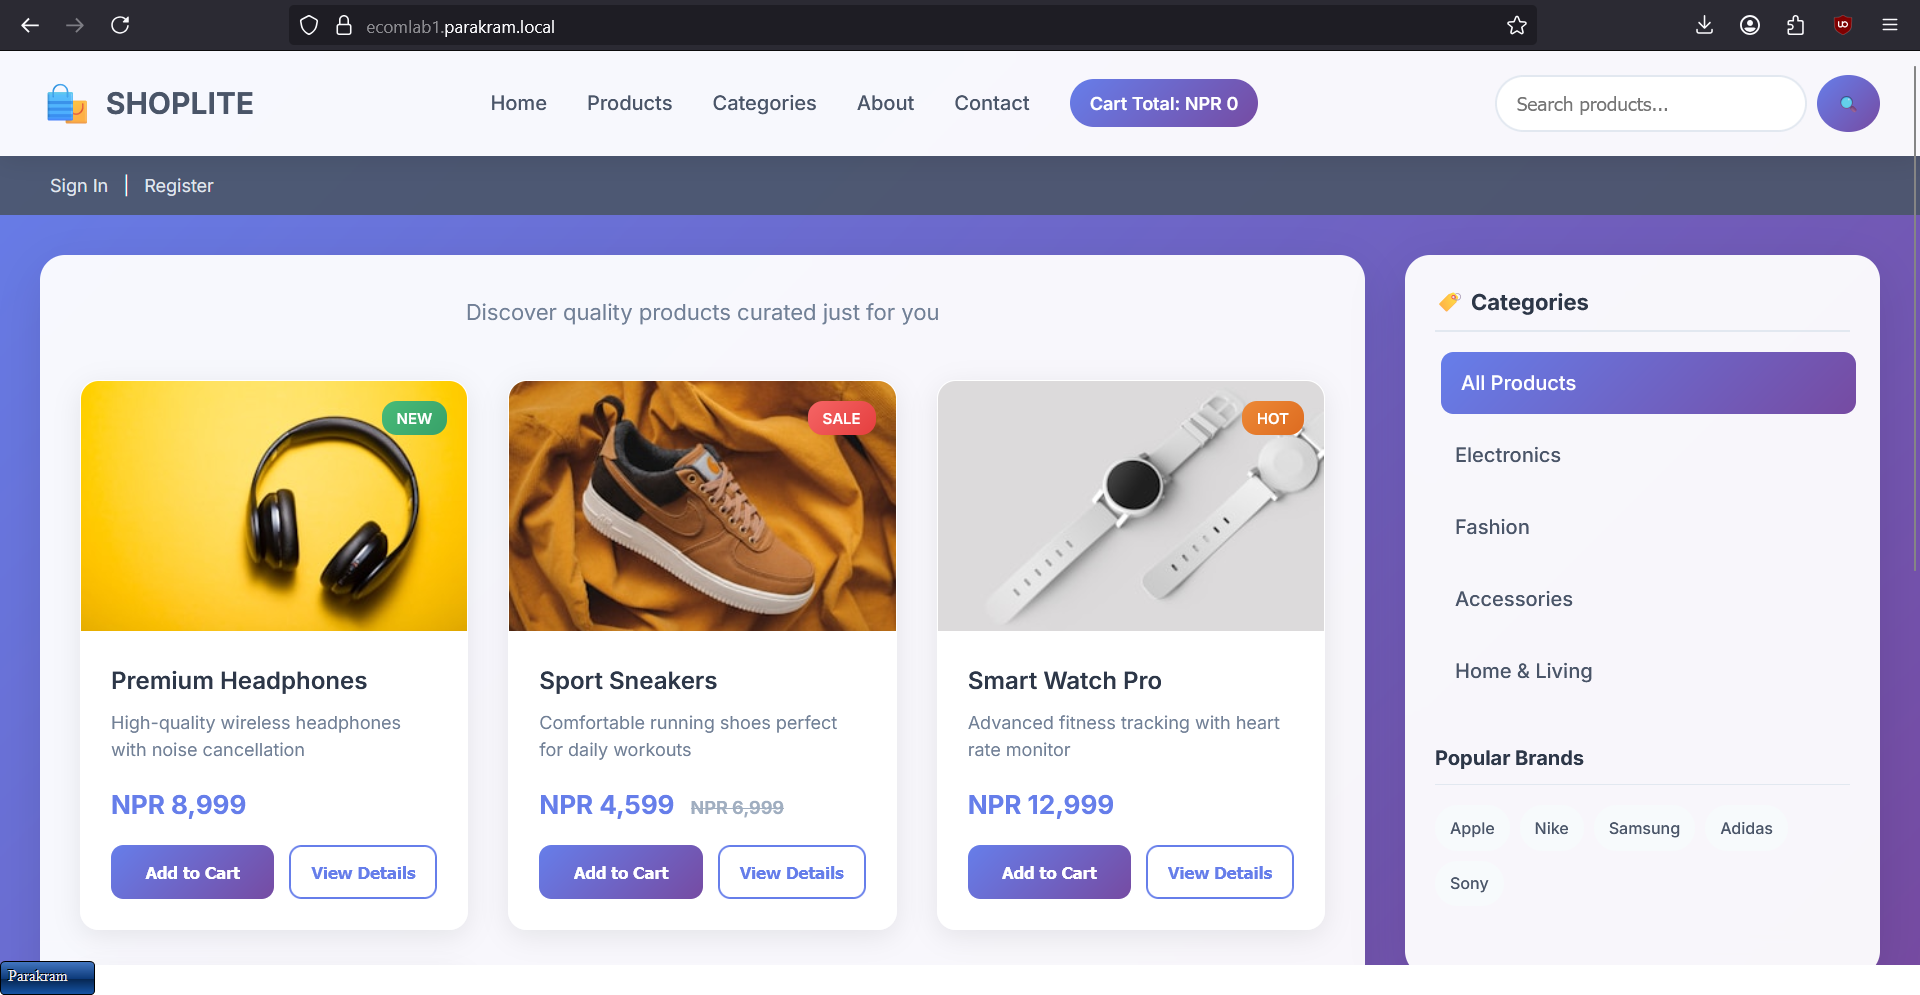
\includegraphics[width=\textwidth]{output.png} 
\end{center}

\section*{7. Result}
The product catalog page was successfully built and displayed, showcasing multiple product items arranged in a grid layout with appropriate styling applied through HTML and CSS.

\section*{8. Conclusion}
This lab covered the basics of building an e-commerce interface, using HTML for page layout and CSS for visual styling. It showed how static product listings can be structured and styled for a clean, user-friendly online presentation.


\section*{9. References}
\begin{itemize}
  \item \href{https://developer.mozilla.org/en-US/docs/Web}{MDN Web Docs}
  \item \href{https://css-tricks.com}{CSS-Tricks}
  \item \href{https://html.spec.whatwg.org/}{HTML Living Standard (WHATWG)}
  \item \href{https://www.w3.org/TR/CSS/#css}{W3C - CSS Standards}
\end{itemize}
\end{document}
